%%%%%%%%%%%%%%%%%%%%%%%%%%%%%%%%%%%%%%%%%
% The Legrand Orange Book
% LaTeX Template
% Version 2.1.1 (14/2/16)
%
% This template has been downloaded from:
% http://www.LaTeXTemplates.com
%
% Original author:
% Mathias Legrand (legrand.mathias@gmail.com) with modifications by:
% Vel (vel@latextemplates.com)
%
% License:
% CC BY-NC-SA 3.0 (http://creativecommons.org/licenses/by-nc-sa/3.0/)
%
% Compiling this template:
% This template uses biber for its bibliography and makeindex for its index.
% When you first open the template, compile it from the command line with the 
% commands below to make sure your LaTeX distribution is configured correctly:
%
% 1) pdflatex main
% 2) makeindex main.idx -s StyleInd.ist
% 3) biber main
% 4) pdflatex main x 2
%
% After this, when you wish to update the bibliography/index use the appropriate
% command above and make sure to compile with pdflatex several times 
% afterwards to propagate your changes to the document.
%
% This template also uses a number of packages which may need to be
% updated to the newest versions for the template to compile. It is strongly
% recommended you update your LaTeX distribution if you have any
% compilation errors.
%
% Important note:
% Chapter heading images should have a 2:1 width:height ratio,
% e.g. 920px width and 460px height.
%
%%%%%%%%%%%%%%%%%%%%%%%%%%%%%%%%%%%%%%%%%

%----------------------------------------------------------------------------------------
%	PACKAGES AND OTHER DOCUMENT CONFIGURATIONS
%----------------------------------------------------------------------------------------

\documentclass[11pt,fleqn]{book} % Default font size and left-justified equations

\usepackage{wasysym}
\usepackage{esint} % various fancy integral symbols
\usepackage{tikz}
\usepackage{tikz-3dplot}
\usepackage{pgfplots}
\pgfplotsset{compat=1.17}
\usetikzlibrary{patterns}
\usepackage{tkz-euclide} 
\usepackage[hyphens]{url}

\usetikzlibrary {arrows.meta} 

\newcommand{\dd}{\mathrm{d}}
\newcommand{\div}{\mathrm{div}}
\newcommand{\rot}{\vv{\mathrm{div}}}
\newcommand{\grad}{\vv{\mathrm{grad}}}

\tikzset{
    support/.style={
        pattern=north east lines,
        draw=none,
        minimum width=0.3,
        minimum height=0.6
    }
    ,>=latex
}

\usepackage[d]{esvect}
%----------------------------------------------------------------------------------------

%SPECIFIC TO THIS CHAPTER
\usepackage{physics}
\usepackage{ifthen}
\usepackage[outline]{contour} % glow around text
\usetikzlibrary{calc} % for pic
\usetikzlibrary{angles,quotes} % for pic
\usetikzlibrary{patterns}
\tikzset{>=latex} % for LaTeX arrow head
\contourlength{1.2pt}

\colorlet{myred}{red!65!black}
\definecolor{myred}{RGB}{55,62,161}
\tikzstyle{ground}=[preaction={fill,top color=black!10,bottom color=black!5,shading angle=20},
                    fill,pattern=north east lines,draw=none,minimum width=0.3,minimum height=0.6]
\tikzstyle{mass}=[line width=0.6,myred,fill=myred!40,rounded corners=1,
                  top color=myred!40,bottom color=myred!20,shading angle=20]
\tikzstyle{rope}=[myred!30,line width=1.2,line cap=round] %very thick

% FORCES SWITCH
\tikzstyle{force}=[->,myred,ultra thick,line cap=round]
\tikzstyle{Fproj}=[force,myred!60]
\newboolean{showforces}
\setboolean{showforces}{true}
%----------------------------------------------------------------------------------------


\input{structure} % Insert the commands.tex file which contains the majority of the structure behind the template

\begin{document}
%----------------------------------------------------------------------------------------
%	TITLE PAGE
%----------------------------------------------------------------------------------------

%\begingroup
%\thispagestyle{empty}
%\begin{tikzpicture}[remember picture,overlay]
%\coordinate [below=12cm] (midpoint) at (current page.north);
%\node at (current page.north west)
%{\begin{tikzpicture}[remember picture,overlay]
%\node[anchor=north west,inner sep=0pt] at (0,0) {
\includegraphics[width=\paperwidth]{background}}; % Background image
%\draw[anchor=north] (midpoint) node [fill=ocre!30!white,fill opacity=0.6,text opacity=1,inner sep=1cm]{\Huge\centering\bfseries\sffamily\parbox[c][][t]{\paperwidth}{\centering Cours de Physique-Chimie\\[15pt] % Book title
%{}\\[20pt] % Subtitle
%{\huge Lycée Baimbridge MP 2025-2026}}}; % Author name
%\end{tikzpicture}};
%\end{tikzpicture}
%\vfill
%\endgroup

%----------------------------------------------------------------------------------------
%	COPYRIGHT PAGE
%----------------------------------------------------------------------------------------

%\newpage
%~\vfill
%\thispagestyle{empty}

%\noindent Copyright \copyright\ CC BY 4.0 2025 Basile Poujol\\ % Copyright notice

%\noindent Licensed under the Creative Commons Attribution-NonCommercial 4.0 Unported License (the ``License''). You may not use this file except in compliance with the License. You may obtain a copy of the License at \url{http://creativecommons.org/licenses/by-nc/3.0}. See the License for the specific language governing permissions and limitations under the License.\\ % License information

%----------------------------------------------------------------------------------------
%	TABLE OF CONTENTS
%----------------------------------------------------------------------------------------

%\usechapterimagefalse % If you don't want to include a chapter image, use this to toggle images off - it can be enabled later with \usechapterimagetrue

\chapterimage{./Pictures/engrenages.jpg} % Table of contents heading image

%\pagestyle{empty} % No headers

%\tableofcontents % Print the table of contents itself

%\cleardoublepage % Forces the first chapter to start on an odd page so it's on the right

%\pagestyle{fancy} % Print headers again



%\part{\'{E}lectromagnétisme}


\setcounter{chapter}{1}

\chapter{Frottements}

Dans le chapitre précédent, nous avons étudié essentiellement les interactions à distance, à travers l'exemple de la gravitation. Comme nous le verrons en électrostatique, la plupart des conclusions établies via la gravitation fonctionnent aussi pour la force électrique de Coulomb qui est également une force centrale conservative.

Cependant, les outils présentés au chapitre 1 décrivent mal les interactions entre deux solides en contact. Celles-ci sont omniprésentes, et nous permettent de marcher, ou bien à une voiture de rouler. Les frottements sont au coeur des problématiques d'ingénierie et dans ce court chapitre nous allons apporter une description simple de ce phénomène.

\section{Force de contact}

Lorsque deux solides sont en contact, des actions mécaniques mutuelles s'exercent. Ces actions sont liées à la présence de forces à l'échelle microscopique agissant au niveau de la surface de contact entre les solides. Ces interaction sont complexes, elles font intervenir en particulier les forces de Van der Waals (cf cours de chimie de MPSI).

Il n'existe pas de loi théorique donnant cette force de contact en fonction de paramètres macroscopiques extérieurs au système. Ainsi, l'étude des forces de contacts est \textbf{phénoménologique} : on s'appuie sur le résultat d'observations et d'expériences.

On décompose donc souvent la réaction de contact de deux solides en deux composantes.

\begin{definition}
    Soient deux solides $S_1$ et $S_2$ en contact. Nous notons $\mathcal{P}$ la plan tangent à la surface de contact $\Sigma$. Les solides exercent l'un sur l'autre une force de réaction $\vv R$ qui se décompose comme suit :
    \begin{equation}
        \vv R = \vv N + \vv T
    \end{equation}
    où :
    \begin{itemize}
        \item $\vv N$ est la composante normale, elle est perpendiculaire au plan  $\mathcal{P}$;
        \item $\vv T$ est la composante tangentielle de la réaction, souvent appelée force de frottement. Elle est contenue dans le plan $\mathcal{P}$.
    \end{itemize}
    La force de réaction s'applique en un point $I$ de la surface de contact, qui ne peut pas être déterminé a priori.
\end{definition}

\begin{figure}[htbp]
    \centering
    \begin{tikzpicture}[scale=2]
  \def\W{2.5}  % ground width
  \def\D{0.2}  % ground depth
  \def\ang{30} % ground angle
  \def\mx{1.5} % mass x position
  \def\w{1.0} % mass x position
  \def\h{0.8} % mass x position
  \def\F{1.25} % force magnitude
  \draw[thick] (0,0) coordinate (O) -- (\ang:\W) coordinate (T) node[anchor=west]{$\mathcal{P}$} ;
  
  \draw[mass,rotate=\ang] (\mx-\w/2,0) rectangle++ (\w,\h) node[anchor=north]{\textcolor{ocre}{$S_2$}};
  \draw[mass,rotate=\ang] (\mx-\w,-\h) rectangle++ (\w,\h) node[anchor=north]{\textcolor{ocre}{$S_1$}};
  
  % FORCES
  \ifthenelse{\boolean{showforces}}{
    \coordinate (F0) at ($(\ang:\mx)+(\ang+90:0.5*\h)$);
    \coordinate (F)  at ($(F0)+(-90:\F)$);
    \coordinate (Fx) at ($(F0)+(\ang-180:{\F*sin(\ang)})$);
    \coordinate (Fy) at ($(F0)+(\ang-90:{\F*cos(\ang)})$);
    
    \draw[force] (\ang:\mx-0.22*\w)++(\ang+90:0.*\h) --++ (\ang+90:{\F*cos(\ang)}) node[anchor=east] {$\vv N_{1 \rightarrow 2}$};
    \draw[force] (\ang:\mx-0.22*\w)++(\ang+90:0.*\h) --++ (\ang:{\F*sin(\ang)}) node[anchor=north] {$\vv T_{1 \rightarrow 2}$};
    \draw[force] (\ang:\mx-0.22*\w)++(\ang+90:0.*\h) --++ (0,\F) node[anchor=east] {$\vv R_{1 \rightarrow 2}$};
    \filldraw[black] (\ang:\mx-0.22*\w) circle (0.03) node[anchor=north]{$I$};
  }{}
  
\end{tikzpicture}
    \caption{Schéma des forces de réaction normale et tangentielle lors d'un contact entre deux solides.}
    \label{fig:contact}
\end{figure}

La composante tangentielle est appelée force de frottement car elle s'oppose au mouvement relatif des deux solides. 

Par ailleurs, pour caractériser le mouvement entre les deux solides, on définit la notion de glissement :

\begin{definition}
    Soient deux solides $S_1$ et $S_2$ en contact au niveau d'un point $O$ et en translation l'un par rapport à l'autre. On définit la vitesse relative de glissement de $S_2$ par rapport à $S_1$ :
    \begin{equation}
        \vv v_g(S_2/S_1) = \vv v(O\in S_1) - \vv v(O \in S_2)
    \end{equation}
    
    On dira que ces solides glissent l'un par rapport à l'autre si cette vitesse de glissement est non nulle.
\end{definition}

\begin{remark}
    La vitesse de glissement entre deux solides présente l'avantage de ne pas dépendre du référentiel choisi. Il est néanmoins important d'exprimer chacune des deux vitesses dans le même référentiel.

    La vitesse de glissement est toujours contenue dans le plan $\mathcal{P}$ du contact entre les solides (sinon les solides ne resteraient pas en contact).
\end{remark}

\section{Lois d'Amontons-Coulomb}

L'étude des forces de frottement s'est faite de manière essentiellement expérimentale. On peut citer notamment Léonard de Vinci, Guillaume Amontons et Charles-Augustin Coulomb qui ont, à partir de nombreuses expériences, abouti aux résultat suivant :

\begin{theorem}[Lois d'Amontons-Coulomb]
    Soient deux solides en contact. L'action $\vv R_{1 \rightarrow 2}$ exercée par le solide 1 sur le solide 2 est décomposée en une composante tangentielle $\vv T$ et une composante normale $\vv N$. On distingue deux cas de figure :
    \begin{itemize}
        \item Si les solides glissent l'un par rapport à l'autre, alors $||\vv T|| = f_d ||\vv N||$ et $\vv T$ est orientée dans le sens opposé à la vitesse de glissement $\vv v_g(S_2/S_1)$
        \item Si les solides ne glissent pas l'un par rapport à l'autre, alors $||\vv T|| < f_s ||\vv N||$
    \end{itemize}
    $f_s$ et $f_d$ sont appelés coefficients de frottement statique et dynamique, respectivement. En général, $f_s > f_d$.
\end{theorem}

\begin{proposition}
    Les coefficients de frottement $f_s$ et $f_d$ sont indépendants de la masse des objets ou de la surface de contact. Ils ne dépendent que du matériau constitutif des deux solides au niveau du contact.
\end{proposition}

\begin{remark}
    Cette propriété est remarquable. On lit dans un article de Christine Blondel et Bertrand Wolff\footnote{\url{http://www.ampere.cnrs.fr/histoire/parcours-historique/lois/coulomb/frottement}} que lors des expériences qui lui ont permis d'établir les lois du frottement, Charles-Augustin Coulomb a fait varier "la nature des matériaux en contact, la charge appliquée, la rugosité et l'étendue des zones de contact, la vitesse de glissement, la durée du contact préalable à l'essai, et encore l'utilisation éventuelle de lubrifiants". Et il a finalement conclu que les coefficients de frottement ne dépendaient principalement que d'un seul paramètre : la nature des matériaux en contact. Une explication microscopique ne viendra que beaucoup plus tard (cf dernière partie de ce chapitre).
\end{remark}

\begin{table}[htbp]
    \centering
    \begin{tabular}{cccc}
    \toprule \\
      Matériau 1 & Matériau 2  & $f_s$ & $f_d$  \\
      \midrule \\
    Glace & Glace & 0.1 & 0.02 \\
    Polyéthylène & Polyéthylène & 0.04 & 0.04 \\
    Polyéthylène & Acier & 0.05 & \\
    Bois & Bois & 0.6 & 0.4 \\
    Acier & Acier & 0.7 & 0.4 \\
    Verre & Verre & 1 & 0.4 \\
    Caoutchouc & Asphalte & 0.9 & 0.7 \\
    Caoutchouc & Caoutchouc & 1.2 & \\
    \bottomrule
    \end{tabular}
    \caption{Quelques coefficients de frottements. On peut remarquer que certains matériaux comme le caoutchouc sont reponsables de beaucoup plus de frottements que d'autres comme le polyéthylène (un plastique). La glace a la propriété particulière $f_s \ll f_d$, c'est-à-dire qu'il est beaucoup plus difficile de la mettre en mouvement que de maintenir un mouvement une fois qu'elle glisse déjà. Source : Engineering Toolbox.}
    \label{tab:coefs_frottement}
\end{table}

\begin{remark}
    En général, $f_d$ et $f_s$ ont des valeurs relativement proches : $f_s \approx f_d$. Ainsi certains énoncés parlent d'un coefficient de frottement $f$ sans préciser s'il s'agit du coefficient de frottement statique ou dynamique ; dans ce cas on suppose que $f_s = f_d = f$.
\end{remark}

\section{Exemples d'application}

Nous allons maintenant voir quelques exemples d'application des lois de Coulomb.

\subsection{Équilibre statique}

\begin{figure}[htbp]
    \centering
    \begin{tikzpicture}[scale=2]
  \def\W{3.5}  % ground width
  \def\D{0.2}  % ground depth
  \def\ang{30} % ground angle
  \def\mx{2.5} % mass x position
  \def\w{1.0} % mass x position
  \def\h{0.8} % mass x position
  \def\F{1.25} % force magnitude
  \draw[thick,top color=blue!20!black!30,bottom color=white,shading angle=\ang+10]
    (0,0) coordinate (O) -- (\ang:\W) coordinate (T) -- ({\W*cos(\ang)},0) coordinate (L) -- cycle;
  %\draw[very thick,white,line cap=round] (0.5*\W,0) --++ (0.15*\W,0) (L)++(0,0.08*\W) --++ (0,0.06*\W);
  \draw[mass,rotate=\ang] (\mx-\w/2,0) rectangle++ (\w,\h);
  \draw pic["$\theta$",draw=black,angle radius=22,angle eccentricity=1.3] {angle=L--O--T};
  
  % FORCES
  \ifthenelse{\boolean{showforces}}{
    \coordinate (F0) at ($(\ang:\mx)+(\ang+90:0.5*\h)$);
    \coordinate (F)  at ($(F0)+(-90:\F)$);
    \coordinate (Fx) at ($(F0)+(\ang-180:{\F*sin(\ang)})$);
    \coordinate (Fy) at ($(F0)+(\ang-90:{\F*cos(\ang)})$);
    \draw[<->,rotate=\ang] (0.25*\W,0.38*\W) node[below=0,left=0] {$\vv{e_x}$}
      -|++ (0.7*\h,0.7*\h) node[anchor=west] {$\vv{e_y}$};
    \draw[force] (\ang:\mx-0.22*\w)++(\ang+90:0.*\h) --++ (\ang+90:{\F*cos(\ang)}) node[anchor=east] {$\vv N$};
    \draw[force] (\ang:\mx-0.22*\w)++(\ang+90:0.*\h) --++ (\ang:{\F*sin(\ang)}) node[anchor=north] {$\vv T$};
    \draw[dashed,ocre!80!black!60] (Fx) -- (F) -- (Fy);
    \draw[Fproj] (F0) -- (Fx) node[anchor=east]  {$mg\sin\theta \vv{e_x}$}; %\vu{x}
    \draw[Fproj] (F0) -- (Fy) node[anchor=west] {$-mg\cos\theta \vv{e_y}$}; %\vu{y}
    \draw[force] (F0) -- (F)  node[anchor=east] {$\vv P$};
    \draw pic["$\theta$",draw=black,angle radius=12,angle eccentricity=1.5] {angle=F--F0--Fy};
    \filldraw[black] (F0) circle (0.03);
    \filldraw[black] (\ang:\mx-0.22*\w) circle (0.03);
  }{}
  
\end{tikzpicture}
    \caption{Masse posée sur un plan incliné.}
    \label{fig:plan_incline}
\end{figure}

\begin{capex}
On considère une masse $m$ posée sur un plan incliné d'un angle $\theta$. Montrer qu'il existe un angle limite au-delà duquel la masse glisse, et calculer cet angle.
\end{capex} 

%La masse est soumise à :
%\begin{itemize}
%    \item Son poids $\vv P$;
%    \item La réaction du support $\vv R = \vv T + \vv N$
%\end{itemize}
%Nous nous plaçons dans le système de coordonnées cartésiennes indiqué dans la figure \ref{fig:plan_incline}. La masse étant à l'équilibre dans le référentiel terrestre supposé galiléen, les forces extérieures se compensent. En projetant l'équilibre des forces sur chacun des deux axes, on obtient :
%\begin{equation}
%    \begin{dcases}
%        ||\vv N|| &= m g \cos \theta\\
%        ||\vv T|| &= m g \sin \theta
%    \end{dcases}
%\end{equation}
%On en déduit que :
%\begin{equation}
%    ||\vv T|| = ||\vv N|| \tan \theta
%\end{equation}
%En utilisant la loi de Coulomb du frottement statique, on obtient alors la condition à laquelle l'équilibre peut être satisfait :
%\begin{equation}
%    \tan \theta < f_s
%\end{equation}
%ce qui est équivalent à $\theta < \theta_s = \arctan f_s$. Il existe ainsi un angle limite au-dessus duquel les frottements ne sont pas suffisants pour maintenir la masse en équilibre, et le solide se met en mouvement.

On peut remarquer que l'angle obtenu est indépendant de la masse du mobile ou de la surface de contact. Il ne dépend que du coefficient de frottement, qui est une propriété des matériaux du support et du mobile.

\subsection{Mise en mouvement}

\begin{figure}[htbp]
    \centering
    \begin{tikzpicture}[scale=2]
  \def\W{3.6}  % ground width
  \def\D{0.2}  % ground depth
  \def\H{1.9}  % human height
  \def\h{0.8}  % mass height
  \def\w{1.0}  % mass width
  \def\mx{0.10*\W} % mass x coordinate
  
  % SETUP
  \draw[ground] (-0.5*\W,0) rectangle++ (\W,-\D);
  \draw (-0.5*\W,0) --++ (\W,0);
  \draw[mass] (\mx,0) rectangle++ (\w,\h) ;
  
  % PERSON
  \coordinate (H) at (0,0.75*\H);
  \draw[thick,line cap=round]
    (H)++(-165:0.3) to[out=-140,in=60]++ (-130:0.3)
    to[out=65,in=-90,looseness=1.0]++ (80:0.45) to[out=90,in=120,looseness=1.4]++ (20:0.2); % pony tail
  \draw[thick,fill=white] (H) circle (0.3);
  \draw[thick,line cap=round] (H)++(-140:0.3) to[out=80,in=-120,looseness=1.8]++ (40:0.6); % hair
  \draw[thick] (H)++(-120:0.3) coordinate (N) to[out=-115,in=40]++ (-130:0.36*\H) coordinate (P);
  \draw[thick,line cap=round] (N)++(-115:0.03) to[out=-60,in=170] (1.04*\mx,\h);
  \draw[thick,line cap=round] (N)++(-115:0.03) to[out=-70,in=170] (\mx,0.92*\h);
  \draw[thick,line cap=round] (P) to[out=-120,in=30,looseness=1.3] (-0.35*\W,0);
  \draw[thick,line cap=round] (P) to[out=-50,in=30,looseness=1.8] (-0.22*\W,0);
  
  % FORCES
  \ifthenelse{\boolean{showforces}}{
    \draw[<->] (\mx+1.4*\w,2.1*\h) node[below=2,left=0] {$\vv{e_z}$}
      |-++ (0.7*\h,-0.7*\h) node[right=0] {$\vv{e_x}$};
    \draw[force] (\mx+0.7*\w,0.) --++ (0, 1.3*\h) node[anchor=west] {$\vv N$};
    \draw[force] (\mx+0.48*\w,0.50*\h) --++ (0,-1.3*\h) node[anchor=west] {$\vv P$};
    \draw[force] (\mx+0.1*\w,0.90*\h) --++ ( 1.4*\h,0) node[anchor=north] {\,$\vv F_{ext}$};
    \draw[force] (\mx+0.7*\w,0.0*\h) --++ (-1.4*\h,0) node[anchor=south] {$\vv T$};
  \filldraw[black] (\mx+0.7*\w,0.) circle (0.05) ;
  \filldraw[black] (\mx+0.5*\w,0.5*\h) circle (0.05) ;  
  }{}
  
\end{tikzpicture}

    \caption{Mise en mouvement d'un solide en contact avec une surface immobile.}
    \label{fig:mise_en_mouvement}
\end{figure}

\begin{capex}
On cherche à mettre en mouvement un objet posé à plat sur un support. Nous supposons qu'une force $\vv F_{ext} = F_{ext} \vv{e_x}$ est appliquée sur un solide de masse $m$. 
Déterminer :
\begin{itemize}
\item La force minimale à appliquer pour mettre le solide en mouvement ;
\item L'accélération du solide une fois qu'il est mis en mouvement.
\end{itemize}
\end{capex}

%Le solide est soumis à son poids $\vv P = m \vv g$, et à la réaction su support $\vv R = \vv T + \vv N$. 
%
%Le principe fondamental de la dynamique, appliqué au solide dans le référentiel du sol supposé galiléen, s'écrit :
%\begin{equation}
%    m \frac{\dd \vv v}{\dd t} = \vv F_{ext} + \vv P + \vv T + \vv N
%\end{equation}
%Projeté selon la verticale, on obtient directement :
%\begin{equation}
%    \vv N = m g \vv{e_z}
%    \label{eq:N}
%\end{equation}
%Ensuite, en projetant selon l'horizontale, et en notant $\vv v = v \vv{e_x}$, on trouve :
%\begin{equation}
%    m \frac{\dd \vv v}{\dd t} \vv{e_x} = F_{ext} \vv{e_x} - \vv T
%    \label{eq:T}
%\end{equation}
%On en déduit que la force de frottement est alignée selon le vecteur $\vv{e_x}$, on note ainsi $\vv T = - T \vv{e_x}$ on distingue deux temps :
%\begin{itemize}
%    \item Dans un premier temps, le solide est à l'équilibre et ne se déplace pas. On a alors $v = 0$ ce qui implique $T = F_{ext}$ et la loi de Coulomb du frottement statique nous donne la condition d'équilibre :
%    \begin{equation}
%        F_{ext} < f_s N = f_s m g
%    \end{equation}
%    Lorsque la force exercée sur le mobile dépasse la force critique $F_c = f_s m g $, la force de frottement ne peut plus compenser la force extérieure appliquée, le mobile se met en mouvement, et on entre dans une phase de glissement.
%    \item Dans cette deuxième phase, le mobile est en glissement. On a alors, par la seconde loi de Coulomb, $T = f_d N$ ce qui se traduit par :
%    \begin{equation}
%        T = f_g m g
%    \end{equation}
%    et le mobile subit une accélération constante :
%    \begin{equation}
%        \frac{\dd v}{\dd t} = \frac{F_{ext}}{m} - f_d g
%    \end{equation}
%    Le mobile continue donc d'accélérer tant que $F_{ext} > f_d m g$, ce qui est le cas au moment de la mise en mouvement puisque $f_d < f_s$
%\end{itemize}

\begin{remark}
    Puisque $f_d < f_s$, on a une discontinuité de la force de frottement qui chute brutalement au moment de la mise en mouvement. Cette discontinuité se ressent parfois lorsque l'on déplace des objets au quotidien, avec une force à exercer plus importante pour mettre un objet en mouvement que pour le déplacer. On le voit particulièrement lorsque l'on déplace un morceau de savon resté longtemps sur une table, on a alors $f_s \gg f_d$.
\end{remark}

\begin{figure}[htbp]
    \centering
    \begin{tikzpicture}[scale=1.3]
  \def\xmax{5.2}
  \def\ymax{2.8}
  \def\xc{0.37*\xmax}
  \def\yc{0.7*\ymax}
  \draw[dashed] (\xc,0) --++ (0,0.97*\ymax); % coordinate (C);
  \draw[ocre!80!black,thick]
    (0,0) -- (\xc,\yc)
    node[scale=0.9,midway,right=5,above=0,rotate={atan2(\yc,\xc)}] {$T = F_{ext} < f_s N$}
    to[out=-90,in=180]++ (0.06*\xmax,-0.08*\xmax) --++ (0.45*\xmax,0)
    node[scale=0.9,midway,below=0] {$T = f_d N$};
  \draw[->,thick] (-0.1*\xmax,0) -- (\xmax,0) node[anchor=south] {$F_{ext}$};
  \draw[->,thick] (0,-0.1*\ymax) -- (0,\ymax) node[anchor=west] {$T$};
  \draw[thick] (\xc,0.1) --++ (0,-0.2) ;
  \node[] at (\xc/2,0.85*\ymax) {équilibre};
  \node[] at ({(\xmax+\xc)/2},0.85*\ymax) {glissement};
  
\end{tikzpicture}
    \caption{\'{E}volution de la force de frottement $T$ en fonction de la force appliquée au mobile pour le faire glisser. On constate une chute de la force de frottement au moment de la mise en mouvement.}
    \label{fig:courbe_frottement}
\end{figure}

\subsection{Freinage}

\begin{capex}
Supposons maintenant qu'après avoir mis en mouvement le mobile à une vitesse initiale $v_0$, on arrête de le pousser. Déterminer la distance parcourue par le mobile avant qu'il ne s'arrête.
\end{capex}

%Dans cette situation, on a toujours un glissement mais la force appliquée est nulle : $F_{ext} = 0$. Les équations \ref{eq:N} et \ref{eq:T} dérivées dans la partie précédente sont toujours valables et on obtient en les combinant :
%\begin{equation}
%    \frac{\dd v}{\dd t} = - f_d g
%\end{equation}
%soit une vitesse qui décroît linéairement :
%\begin{equation}
%    v(t) = v_0 - f_d g t
%\end{equation}
%Ainsi le mobile va continuer à avancer jusqu'à l'instant $t_f = \frac{v_0}{f_d g}$ pour lequel la vitesse s'annule. 
%La distance parcourue est alors :
%\begin{equation}
%    L = \int_0^{t_f} v(t) \dd t = \int_0^{t_f} (v_0 - f_d g t) \dd t = v_0 t_f - f_d g \frac{t_f^2}{2} = \frac{v_0^2}{2 f_d g}
%\end{equation}

On constate que cette distance est d'autant plus importante que la vitesse initiale est élevée et que le coefficient de frottement dynamique est faible. Une fois cette distance parcourue, le mobile s'arrête, et on se retrouve dans une situation d'équilibre où la loi du frottement statique est à nouveau vérifiée.

\section{Aspects énergétiques}

Nous nous intéressons maintenant aux aspects énergétiques de la force de frottement. 

Lorsque deux solides ne glissent pas l'un par rapport à l'autre (situation d'adhérence), la force de frottement ne travaille pas ($\vv{\dd \ell} = \vv 0$ et $\delta W = \vv T \cdot \vv{\dd \ell}$).

Lorsque les solides glissent l'un par rapport à l'autre, la force de frottement est colinéaire et de sens opposé au glissement, il s'agit donc d'une force qui travaille et dont le travail est négatif : elle dissipe de l'énergie sous forme de chaleur.

Prenons l'exemple de la mise en mouvement et du freinage que nous venons de voir. Le travail de la force de frottement au cours de la trajectoire du mobile s'écrit :
\begin{equation}
    W = \int_\mathcal{C} \vv T \cdot \vv{\dd \ell}
\end{equation}
où $\mathcal{C}$ est le chamin suivi par le mobile.

Comme le travail n'est positif que lorsque le mobile glisse, la loi de Coulomb dynamique est vérifiée et on a $|| \vv T|| = f_d || \vv N||$. Par ailleurs comme $\vv T$ est toujours colinéaire à $\vv{\dd \ell}$ et de direction opposée :
\begin{equation}
    \vv T \cdot \vv{\dd \ell} = - || \vv T|| \dd \ell
\end{equation}
Enfin, on a vu que l'équilibre des forces dans la direction verticale impose $N = mg$ ce qui implique que :
\begin{equation}
    W = \int_{\mathcal{C}} - || \vv T|| \dd \ell = - \int_{\mathcal{C}} f_d || \vv N|| \dd \ell = - f_d mg L
\end{equation}
où $L$ est la longueur totale du chemin suivi. Le travail de la force dépend du chemin suivi si bien que :

\begin{proposition}
    La force de frottement n'est pas une force conservative.
\end{proposition}

Ainsi, pour minimiser les frottements, on a intérêt à minimiser la longueur du chemin suivi, c'est-à-dire à déplacer les objets en ligne droite.

\begin{capex}
Retrouver la distance parcourue par le mobile lors du freinage en utilisant une méthode énergétique.
\end{capex}

%On peut utiliser l'argument énergétique pour résoudre le problème du freinage. En effet, la variation d'énergie mécanique du mobile correspond au travail des forces non conservatives :
%\begin{equation}
%    \Delta (E_p + E_c) = W_{nc}
%\end{equation}
%Ici l'énergie potentielle de pesanteur est constante le long de la trajectoire, et la seule force non conservative qui travaille est la force de frottement $\vv T$. On obtient donc :
%\begin{equation}
%    - \frac{1}{2} m v_0^2 = - f_d m g L
%\end{equation}
%où $L$ est la distance parcourue par le mobile, ce qui fournit directement la relation que nous avons déjà dérivée :
%\begin{equation}
%    L = \frac{v_0^2}{2 f_d g}
%\end{equation}
%
%Autrement dit, la distance parcourue par le mobile est le résultat de l'équilibre entre l'énergie cinétique initiale du mobile et la consommation de cette énergie par le travail des forces de frottement.

\section{Interprétation microscopique}

Il est surprenant que la force de frottement soit indépendante de la surface macroscopique de contact, mais ne dépende que de la norme de la composante normale de la réaction. Cette propriété est contre-intuitive, mais a été prouvée de manière expérimentale. Comment l'expliquer ?

Pour la comprendre, nous pouvons analyser la surface de contact à l'échelle microscopique. Tous les solides présentent des aspérités de taille micrométrique, et la surface de contact réelle entre deux solides est bien plus faible que la surface de contact apparente. Ce sont ces aspérités qui sont responsables de la force de frottement.

\begin{figure}[htbp]
    \centering
    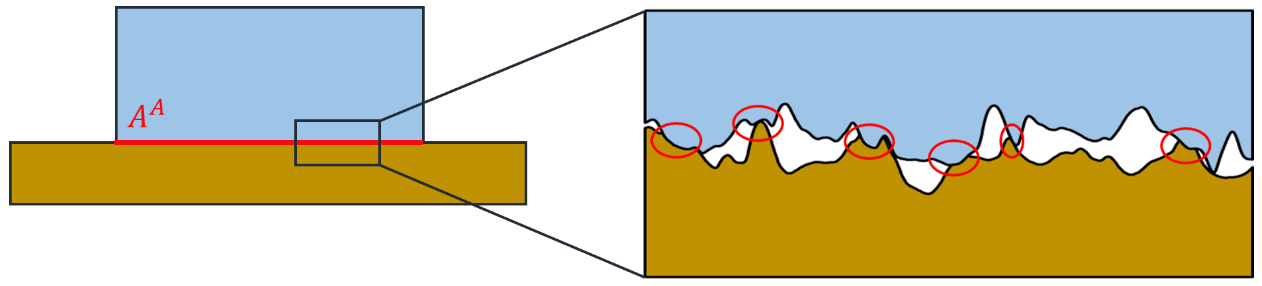
\includegraphics[width=0.9\linewidth]{Pictures/contact_solides_zoom.png}
    \caption{Zoom à l'échelle microscopique sur la surface de contact entre deux solides. Figure issue de la thèse d'Antoine Aymard.}
    \label{fig:contact_micro}
\end{figure}

Lorsqu'une force normale est exercée par un solide sur l'autre, les aspérités sont comprimées et se déforment sous l'effet de la pression. La surface réelle de contact augmente, ce qui augmente les forces de Van der Waals et augmente ainsi la force de frottement. On retrouve donc le comportement attendu. En d'autres termes, la force de frottement ne dépend pas de la surface de contact macroscopique, mais elle dépend de la surface réelle de contact à l'échelle microscopique, qui est fixée par la réaction normale du support.

\begin{encart}
Si aujourd'hui, on sait produire des matériaux avec un très fort ou un très faible coefficient de frottement, il est plus difficile de créer des matériaux avec un coefficient de frottement intermédiaire que l'on puisse contrôler.

 Les travaux de recherches menés à l'école centrale de Lyon par Antoine Aymard, Émilie Delplanque, Davy Dalmas et Julien Scheibert, se sont inspirés de l'interprétation microscopique du frottement solide afin de contrôler le coefficient de frottement d'une surface. Ils essayent de reproduire de façon artificielle et contrôlable des aspérités sur une surface en silicone.
 
 En couvrant cette surface de calottes sphériques de différentes tailles, et de différentes hauteurs, les scientifiques ont pu montrer que le coefficient de frottement était modulé par la densité et les hauteurs des aspérités. Pour une configuration donnée, la surface de contact augmente avec la force normale appliquée sur le support, ce qui augmente la force de frottement conformément à la loi de Coulomb.

 Référence de l'article : Aymard, Antoine, Delplanque, Emilie, Dalmas, Davy, \& Scheibert, Julien (2024). Designing metainterfaces with specified friction laws. Science, 383(6679), 200-204.

 Vidéo sur le site du CNRS :  \url{https://www.insis.cnrs.fr/fr/cnrsinfo/designer-les-interfaces-de-contact-du-frottement-la-demande}
\end{encart}

\begin{figure}[htbp]
    \centering
    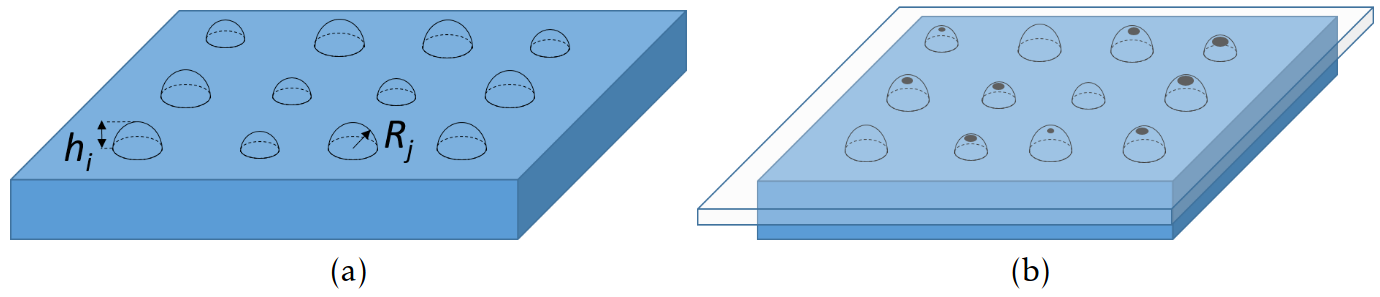
\includegraphics[width=\linewidth]{Pictures/surface_spheres.png} 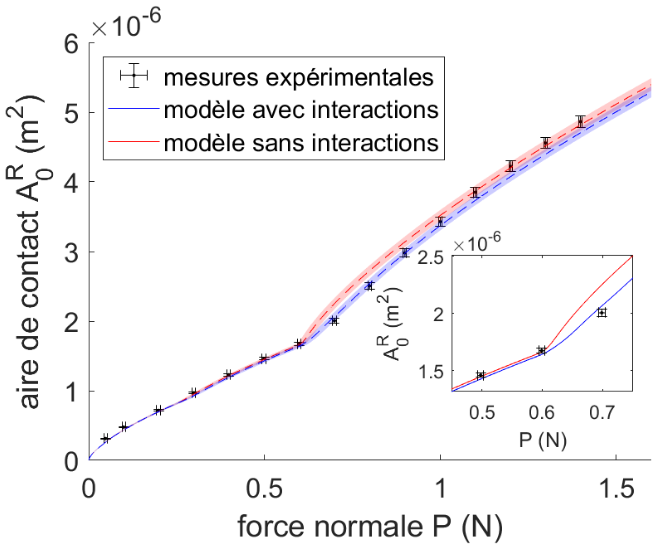
\includegraphics[width=0.5\linewidth]{Pictures/surface_reelle_de_contact.png}
    \caption{En haut : exemples de surfaces en silicone fabriquées par l'équipe de l'école Centrale de Lyon pour contrôler le coefficient de frottement. En bas : pour l'une des surfaces, la surface réelle de contact est tracée en fonction de la force normale appliquée sur l'échantillon. Source : thèse de Antoine Aymard.}
    \label{fig:exemple_centrale}
\end{figure}


\end{document}
